\begin{figure}[p]
\centering
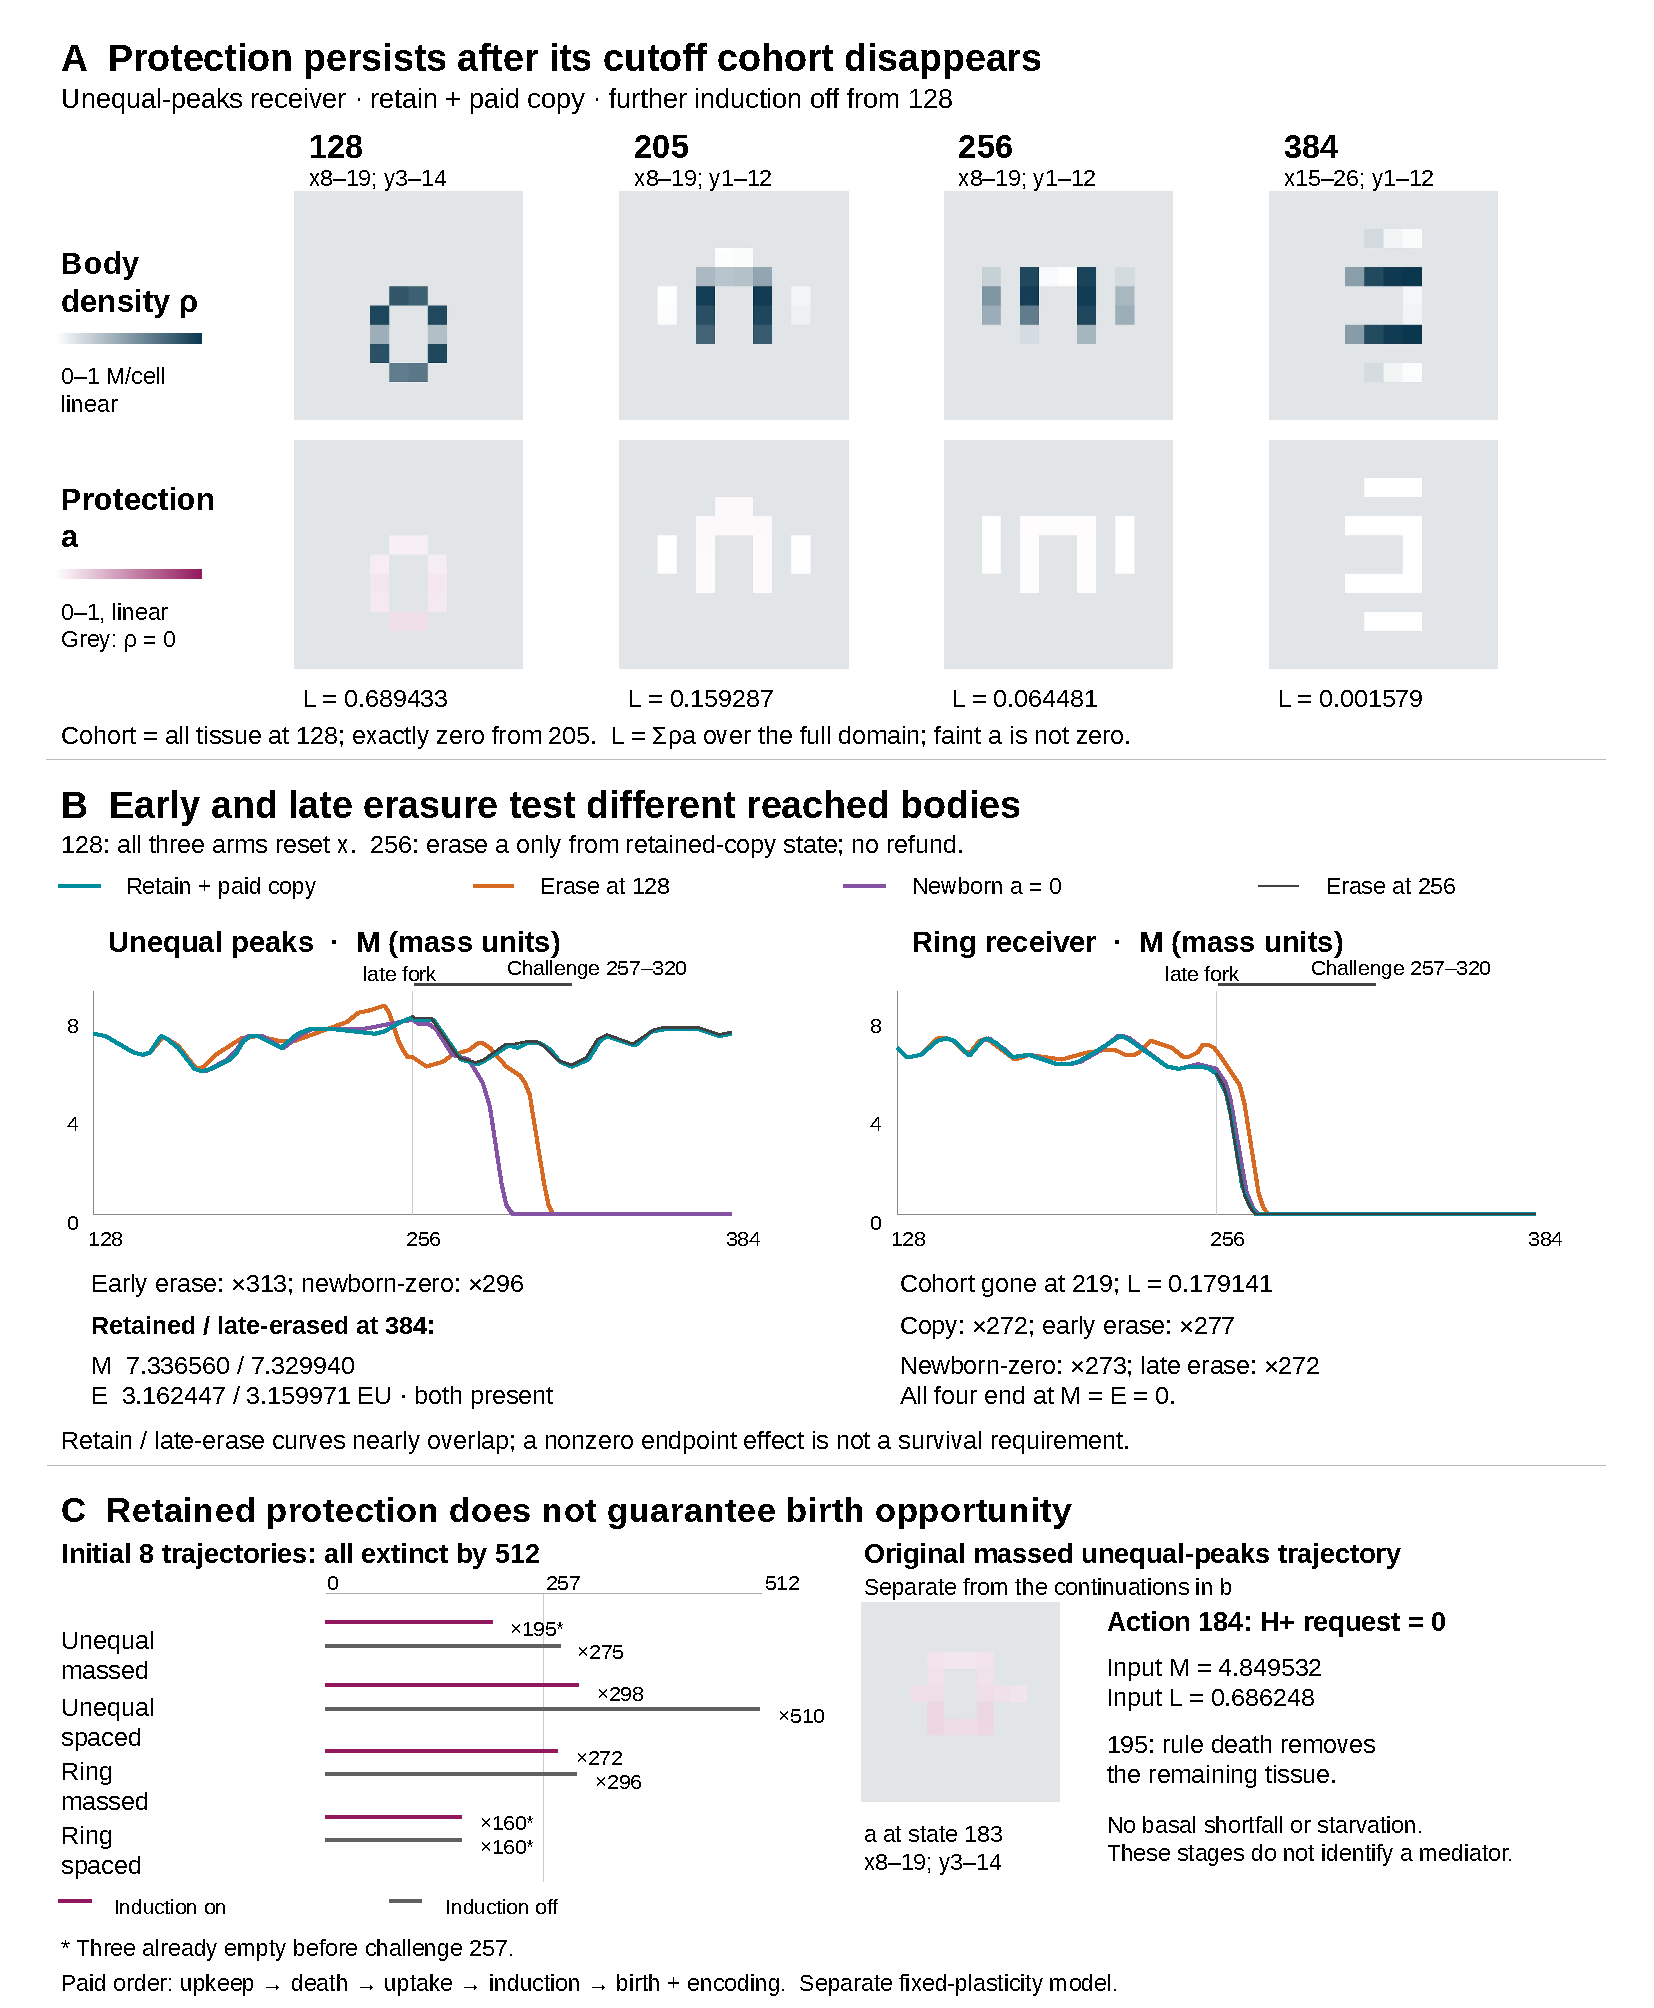
\includegraphics[width=0.95\linewidth]{figures/main/protection/paid_protection_renewal.pdf}
\caption{\textbf{Transmission across tissue replacement and the necessity of residual protection are different questions.}
\textbf{a,} Archived unequal-peaks fields under retained paid copying. All tissue present at cutoff 128 disappears by 205, while load $L=\sum\rho a$ remains nonzero. Each column shows density and protection in one labelled original-coordinate window; both use fixed linear 0--1 scales, with empty cells grey. Further induction is off.
\textbf{b,} Six early continuations and two late-erasure futures, including extinct tails. Early branches share each physical receiver and reset the fast sensor. Late erasure clears only protection at retained-copy state 256, without a refund; retained references are reused. Unequal peaks persist to 384 under both late conditions despite a quantitative difference. The ring loses its cutoff cohort but subsequently fails under all four conditions.
\textbf{c,} All eight original trajectories fail; three are empty before challenge. In the original massed unequal-peaks trajectory, positive birth opportunity disappears at 184 despite protection, before rule death empties the body at 195. This is a separate trajectory from b. Copying and erasure change costs and coupled development; these comparisons identify neither an information-only effect nor a mediator or general adaptation.}
\label{fig:paid-protection-renewal}
\end{figure}
